\documentclass{../res/univ-projet}

%Import des packages utilisés pour le document
\usepackage[utf8x]{inputenc}
\usepackage[francais]{babel}
\usepackage[T1]{fontenc}

%Redéfinition des marges
\addtolength{\topmargin}{-1cm}
\addtolength{\textheight}{1cm}
\addtolength{\headsep}{0.8cm}
\addtolength{\footskip}{-0.2cm}

%Variables
\logo{../res/logo_univ.png}
\title{Document d'architecture du logiciel}
\author{Matthieu \bsc{Fin}, Guillaume \bsc{Leroy}}
\projet{GPG}
\projdesc{Interface Graphique GPG}
\filiere{M1SSI - Conduite de Projet}
\version{0.1}
\relecteur{}
\signataire{Magali \bsc{Bardet}}
\date{\today}


\histentry{0.1}{23/11/2014}{Version initiale.}

% Definition de couleurs :
% Couleur de fond des nom de classes
\definecolor{classColor}{rgb}{.20,.42,.57}
% Couleur de fond des noms de methode
\definecolor{methodeColor}{rgb}{.38,.62,.81}
% Couleur de fond des legends (Nom, Entrée, precondtion, sortie, postcondition, description)
\definecolor{legendColor}{rgb}{.45,.58,.67}



% Commande permettant de créer un tableau entrées / sortie / pré-post conditions pour les méthodes
%\newcommand{\methode}[6]{
%  \begin{tabular}{|>{\centering}p{2.5cm}|>{\centering}p{7cm}|}
%    \hline
%    \color{white}\cellcolor{legendColor}\bfseries{Nom}&
%    #1 \cr
%    \hline
%    \color{white}\cellcolor{legendColor}\bfseries{Entrée}&
%    #2 \cr
%    \hline
%    \color{white}\cellcolor{legendColor}\bfseries{Préconditions}&
%    #3 \cr
%    \hline
%    \color{white}\cellcolor{legendColor}\bfseries{Sortie}&
%    #4 \cr
%    \hline
%    \color{white}\cellcolor{legendColor}\bfseries{Postconditions}&
%    #5 \cr
%    \hline
%    \color{white}\cellcolor{legendColor}\bfseries{Description}&
%    #6 \cr
%    \hline
%  \end{tabular}\\
%}


% Commande permettant de créer un tableau entrées / sortie / pré-post conditions pour les méthodes
% N'affiche pas les champs vide...
\newcommand{\methode}[6]{
  \def\vide{} \def\tempa{#1} \def\tempb{#2} \def\tempc{#3} \def\tempd{#4} \def\tempe{#5} \def\tempf{#6}
  \def\casa{\ifx\empty\tempa \else \hline \color{white}\cellcolor{legendColor}\bfseries{Nom}            & #1 \cr \fi }
  \def\casb{\ifx\empty\tempb \else \hline \color{white}\cellcolor{legendColor}\bfseries{Entrée}         & #2 \cr \fi }
  \def\casc{\ifx\empty\tempc \else \hline \color{white}\cellcolor{legendColor}\bfseries{Préconditions}  & #3 \cr \fi }
  \def\casd{\ifx\empty\tempd \else \hline \color{white}\cellcolor{legendColor}\bfseries{Sortie}         & #4 \cr \fi }
  \def\case{\ifx\empty\tempe \else \hline \color{white}\cellcolor{legendColor}\bfseries{Postconditions} & #5 \cr \fi }
  \def\casf{\ifx\empty\tempf \else \hline \color{white}\cellcolor{legendColor}\bfseries{Description}    & #6 \cr \fi }
  %\begin{tabular}{|>{\centering}p{2.5cm}|>{\centering}p{7cm}|}
  \begin{tabular}{|>{\centering}p{2.5cm}|>{\centering}p{9cm}|}
    \casa \casb \casc \casd \case \casf
    \hline
  \end{tabular}
}

% Commande pour definir une methode dans une \class
\newcommand{\methodeclass}[6]{
  & \color{white}\cellcolor{methodeColor}\bfseries{#1} & \cr
  & \methode{}{#2}{#3}{#4}{#5}{#6} & \cr
  & & \cr
}

% Commande permettant de regrouper des methode dans un tableau portant le nom de la classe.
\newcommand{\class}[2]{%
  \begin{tabular}{|c c c|}
    \hline
    \multicolumn{3}{|>{\color{white}\columncolor{classColor}}c|}{\bfseries{#1}} \cr
    \hline
    & & \cr
    #2
    \hline
  \end{tabular}\\  
}


% -- Début du document -- %
\begin{document}

%Page de garde
\maketitle
\newpage
%La table des matières
\tableofcontents
\newpage

\section{Objet}
  Ce document permet d'établir une vue globale de l'architecture logicielle envisagée pour la conception d'une interface graphique reposant sur le logiciel GnuPG de façon à simpliciter son utilisation pour un utilisateur débutant mais toutefois en laissant apparaitre les fonctionnalités avancées pour un utilisateur expérimenté. Il décrit comment concevoir cette interface pour répondre aux spécifications du client ainsi qu'une conception détaillée des différents modules nécessaires à son bon fonctionnement. 

\section{Documents applicables et de référence}
  \begin{itemize}
    \item La spécification technique des besoins
  \end{itemize}

\section{Terminologie et sigles utilisés}
  \subsection{Acronymes}
    \begin{itemize}
      \item GNOME GNU Network Object Model Environment
      \item GNU GNU's Not UNIX
      \item IETF Internet Engineering Task Force
      \item KDE K Desktop Environment
      \item MVC Model View Controller
      \item PGP Pretty Good Privacy
      \item RFC Request For Comments
    \end{itemize}

  \subsection{Glossaire}
    \begin{itemize}
      \item C++\\
        Langage de programmation compilé.
      \item Environement de bureau\\
        Ensemble de programmes qui permettent de manipuler le système à travers une interface graphique.
      \item MVC\\
        Patron de conception répondant aux besoins des applications intéractives en séparant les problèmatiques en trois parties :
        \begin{itemize}
          \item Le modèle\\
            Il représente les données manipulées par l'application et est responsable de leur intégrité.
          \item La vue\\
            Ce avec quoi l'utilisateur interagit. Sa fonction principale est d'afficher les données envoyées par le modèle.
          \item Le controller\\
            Il traite les évenements et met à jour la vue ou le modèle selon l'action effectuée.
        \end{itemize}
      \item Qt\\
        Interface de programmation orientée objet développée en C++ permettant la conception simple d'interface graphique compatible GNU Linux / Windows / Mac OS X.
    \end{itemize}

\section{Configuration requise}
  \subsection{Système d'exploitation}
    GNU Linux
  \subsection{Logiciels}
    Environement de bureau KDE (v4.0 ou ultérieure) ou GNOME (v3.0 ou ultérieure)\\
    GnuPG (v1.4 ou ultérieure)
  \subsection{Matériel}
    Aucune configuration minimale n'est demandée.

\section{Architecture statique}
  \subsection{Structure} % (fold)
    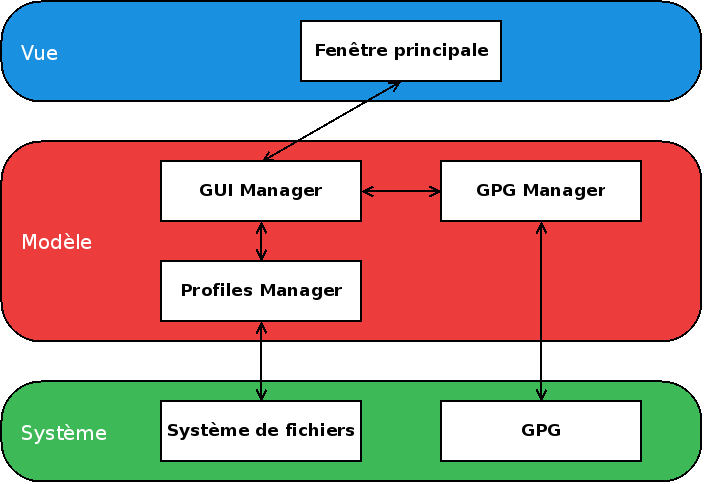
\includegraphics[scale=0.5]{graphics/diagramme_archi.png}
  \subsection{Description des classes} % (fold)
      \subsubsection{Profile}
        \class{Profile}{
          \methodeclass
            {getID}
            {}
            {}
            {Entier représentant l'identifiant unique du profil}
            {}
            {Renvoie l'identifiant unique du profil}
          \methodeclass
            {getName}
            {}
            {}
            {QString représentant le nom du profil}
            {}
            {Renvoie le nom du profil}
          \methodeclass
            {getPath}
            {}
            {}
            {QString représentant le chemin absolu vers le dossier de configuration de GPG}
            {}
            {Renvoie le chemin absolu vers le dossier de configuration}
          \methodeclass
            {setPath}
            {path : QString}
            {path référence un dossier de configuration de GPG valide}
            {}
            {QString représentant le chemin vers le dossier de configuration de GPG du profil est changé}
            {Change le dossier de configuration de GPG du profil}
        }

%        \methode
%        {getID}
%        {}
%        {}
%        {Entier représentant l'identifiant unique du profil}
%        {}
%        {Renvoie l'identifiant unique du profil}
%        
%        \methode
%        {getName}
%        {}
%        {}
%        {QString représentant le nom du profil}
%        {}
%        {Renvoie le nom du profil}
%        
%        \methode
%        {getPath}
%        {}
%        {}
%        {QString représentant le chemin absolu vers le dossier de configuration de GPG}
%        {}
%        {Renvoie le chemin absolu vers le dossier de configuration}
%        
%        \methode
%        {setPath}
%        {path : QString}
%        {path référence un dossier de configuration de GPG valide}
%        {}
%        {QString représentant le chemin vers le dossier de configuration de GPG du profil est changé}
%        {Change le dossier de configuration de GPG du profil}

      \subsubsection{ProfileManager}
        \class{ProfileManager}{
          \methodeclass
          {getPath}
          {}
          {}
          {QString représentant le chemin absolu vers le fichier de configuration de l'application}
          {}
          {Renvoie le chemin absolu vers le fichier de configuration de l'application}
        
          \methodeclass
          {profileAvailable}
          {p : Profile}
          {}
          {Booléen ayant pour valeur vrai si p est libre d'utilisation, faux sinon}
          {Vrai si p n'est utilisé par aucune autre fenêtre de l'application}
          {Renvoie vrai si p est libre, faux sinon}
          
          \methodeclass
          {getProfiles}
          {}
          {}
          {La liste de tous les profils}
          {QList<Profile> contenant tous les profils présents dans le fichier de configuration de l'application}
          {La liste de tous les profils présents dans le fichier de configuration de l'application}
          
          \methodeclass
          {save}
          {}
          {}
          {}
          {La liste des profils est sauvegardée dans le fichier de configuration de l'application}
          {Sauvegarde la liste des profils dans le fichier de configuration de l'application}
          
          \methodeclass
          {runProfile}
          {id : Entier}
          {id est positif ou nul, il correspond à un identifiant de profil et ce profil doit être libre d'utilisation}
          {}
          {Une nouvelle fenêtre est ouverte avec le profil ayant pour identifiant id}
          {Ouvre une nouvelle fenêtre avec le profil donné}
          
          \methodeclass
          {load}
          {}
          {}
          {}
          {Les profils présents dans le fichier de configuration de l'application sont chargés}
          {Charge les profils présents dans le fichier de configuration de l'application}
          
          \methodeclass
          {createProfile}
          {name : QString\\path : QString}
          {name n'est pas vide\\path référence un dossier de configuration de GPG valide}
          {Profile représentant le profil créé}
          {Un objet Profile est créé et il est ajouté à la liste des profils}
          {Crée un profil, l'ajoute à la liste des profils et retourne l'objet Profil créé}
          
          \methodeclass
          {setProfilePath}
          {p : Profile\\path : QString}
          {path est un chemin absolu référençant un dossier de configuration de GPG valide}
          {}
          {Le chemin de p est changé}
          {Change le dossier de configuration lié à p}
          
          \methodeclass
          {changeProfile}
          {p : Profile}
          {p est un profil libre d'utilisation}
          {}
          {Le profil de la fenêtre courante est changé}
          {Change le profil associé à la fenêtre courante}
        }
      \subsubsection{Action}
        \class{Action}{
          \methodeclass
          {getCmd}
          {}
          {}
          {QString représentant le nom de la commande GPG}
          {}
          {Retourne le nom de la commande GPG}
          
          \methodeclass
          {getOptions}
          {}
          {}
          {QStringList contenant les options de la commande GPG}
          {}
          {Retourne la liste des options de la commande GPG}
          
          \methodeclass
          {getInteractions}
          {}
          {}
          {QStringList contenant les intéractions utilisateur durant l'exécution de la commande}
          {}
          {Retourne la liste des intéractions utilisateur durant l'exécution de la commande}
          
          \methodeclass
          {getArgs}
          {}
          {}
          {QStringList content les arguments de la commande GPG}
          {}
          {Retourne la liste des arguments de la commande GPG}
          
          \methodeclass
          {hasInteraction}
          {}
          {}
          {Booleen ayant pour valeur vrai s'il reste des interactions utilisateur}
          {}
          {Retourne vrai s'il reste des interactions utilisateur}
          
          \methodeclass
          {nextInteraction}
          {}
          {hasInteraction()}
          {QString représentant l'interaction utilisateur courante}
          {L'interaction utilisateur courante devient l'interaction utilisateur suivante}
          {Retourne l'interaction utilisateur suivante}
        }
        
        \subsubsection{QuestionType}
        Énumération des différents types de questions :
        \begin{itemize}
          \item NO\_QUESTION
          \item CLOSED\_QUESTION
          \item OPENED\_QUESTION
        \end{itemize}
        
        \subsubsection{GPGManager}
          \class{GPGManager}{
          \methodeclass
          {isRunning}
          {}
          {}
          {Boolean ayant pour valeur vrai si l'exécution de l'action par GPG est en cours}
          {}
          {Retourne vrai si l'exécution de l'action par GPG est en cours}
          
          \methodeclass
          {getQuestionType}
          {}
          {isRunning()}
          {QuestionType représentant le type de la dernière question posée par GPG}
          {}
          {Retourne le type de a dernière question posée par GPG}
          
          \methodeclass
          {getAction}
          {}
          {}
          {Action représentant l'action à exécuter par GPG}
          {}
          {Retourne l'action à exécuter par GPG}
          
          \methodeclass
          {execute}
          {}
          {!isRunning()}
          {}
          {GPG a exécuté l'action associée au manager}
          {Exécute l'action associé au manager}
          
          \methodeclass
          {setAction}
          {a : Action}
          {!isRunning()}
          {}
          {L'action associée au manager a été changé}
          {Change l'action à exécuter par GPG associée au manager}
        
          \methodeclass
          {getOutput}
          {}
          {!isRunning()}
          {QString représentant la sortie de GPG}
          {Contient la sortie de GPG}
          {Retourne la sortie de GPG}
        }
        
        \subsubsection{Instance}
          \class{Instance}{
            \methodeclass
            {getProfile}
            {}
            {}
            {Profile}
            {}
            {Retourne le profil associé à l'instance}
          }
          
        \subsubsection{GPGKeyLevel}
          \class{GPGKeyLevel}{
            \methodeclass
            {getName}
            {}
            {}
            {QString représentant le nom du niveau}
            {}
            {Retourne le nom du niveau}
            
            \methodeclass
            {getLevel}
            {}
            {}
            {Entier représentant le niveau}
            {}
            {Retourne le niveau}
          }
          
        \subsubsection{GPGKey}
          \class{GPGKey}{
          \methodeclass
          {getSubKeys}
          {}
          {}
          {QList<GPGKey> contenant les sous clés de cette clé}
          {}
          {Retourne la liste des sous clés de cette clé}
          
          \methodeclass
          {getEmail}
          {}
          {}
          {QString représentant l'email associé à la clé}
          {}
          {Retourne l'email associé à la clé}
          
          \methodeclass
          {getName}
          {}
          {}
          {QString représentant le nom du propriétaire de la clé}
          {}
          {Retourne le nom du propriétaire de la clé}
          
          \methodeclass
          {getCreationDate}
          {}
          {}
          {QDate représentant la date de création de la clé}
          {}
          {Retourne la date de création de la date}
          
          \methodeclass
          {getID}
          {}
          {}
          {QString représentant l'ID de la clé}
          {}
          {Retourne l'ID de la clé}
          
          \methodeclass
          {getComments}
          {}
          {}
          {QString représentant les commentaires de la clé}
          {}
          {Retourne les commentaires de la clé}
          
          \methodeclass
          {getTrust}
          {}
          {}
          {GPGKeyLevel représentant le niveau de confiance de la clé}
          {}
          {Retourne le niveau de confiance de la clé}
          
          \methodeclass
          {getValidity}
          {}
          {}
          {GPGKeyLevel représentant le niveau de validité de la clé}
          {}
          {Retourne le niveaude validité de la clé}
          
          \methodeclass
          {addSubKey}
          {k : GPGKey}
          {}
          {}
          {}
          {Ajoute une sous clé à cette clé}
          
          \methodeclass
          {removeSubKey}
          {k : GPGKey}
          {k est une sous clé de cette clé}
          {}
          {}
          {Supprime k des sous clés de cette clé}
          
          \methodeclass
          {setTrust}
          {t : GPGKeyLevel}
          {}
          {}
          {Le niveau de confiance de cette clé vaut t}
          {Change le niveau de confiance de cette clé}
        }
          
        \subsubsection{GPGKeyManager}
          \class{GPGKeyManager}{
            \methodeclass
            {getKeys}
            {}
            {}
            {QList<GPGKey> contenant toutes les clés appartenant au trousseau}
            {}
            {Retourne la liste de toutes les clés appartenant au trousseau}
            
            \methodeclass
            {createKey}
            {email : QString\\name : QString\\comments : QString}
            {}
            {GPGKey}
            {Une clé est crée et elle est ajoutée au trousseau}
            {Génére une clé, l'ajoute au trousseau et la retourne}
            
            \methodeclass
            {deleteKey}
            {k : GPGKey}
            {k fait partie du trousseau}
            {}
            {}
            {Supprime une clé du trousseau}
        }
           
  % subsection justification_techniques (end)
\section{Fonctionnement dynamique} % (fold)
\label{sec:fonctionnement_dynamique}

  \textcolor{blue}{
    TODO : \\
    Pour les principaux scénarii identifiés dans la spécification technique de besoin.
    \begin{itemize}
      \item Liste des composants mis en jeu.
      \item Description du processus de mise en oeuvre sous la forme d'une
      séquence d'appels aux services offerts par les différents composants et en faisant
      clairement apparaître
      \begin{itemize}
        \item la logique et le flux des événements traités
        \item les interactions du logiciels avec les acteurs
        \item les interactions entre les composants au travers de leurs interfaces
      \end{itemize}
    \end{itemize}
  }

% section fonctionnement_dynamique (end)
\section{Traçabilité} % (fold)
\label{sec:tra_abilit_}

  \textcolor{blue}{
    TODO : \\
    Récapitulatif des liens de dépendance entre les constituants du logiciel et les exigences de
    la STB (par exemple sous forme de tableau).
  }

% section tra_abilit_ (end)
\end{document}

